\subsection{Dataset}

Cityscapes is a large-scale dataset widely used for training, evaluating and benchmarking algorithms in the fields of computer vision, particularly for models used to perform semantic segmentation as well as instance segmentation of urban street scenes. It consists of high resolution images captured from a vehicle-mounted camera while driving through 50 different cities in Germany and neighbouring countries. The capturing apparatus is equipped with a dual lens which gives it stereoscopic capability, allowing for the possibility of applying stereo vision techniques useful for additional tasks like depth estimation, 3D reconstruction and scene understanding. 

The scenes in the CityScapes dataset represent a variety of urban settings, seasons, daylight conditions, and weather scenarios, providing robust, real-world environments for training models that need to perform under varied conditions. This dataset has been widely used in research for developing, testing and benchmarking new algorithms for computer vision tasks, gaining a place alongside datasets as iconic as ImageNet, COCO and Pascal VOC. The Cityscapes dataset can be accessed in the following address:
\begin{center}
\url{https://www.cityscapes-dataset.com}
\end{center}

The images that are used for our analysis are located in the folder \small\texttt{data/leftImg8bit}. These, as the name suggests, are taken from the left lens of the stereo camera system. They form the main high-resolution images (2,048$\times$1,024 pixels) with an 8-bit color depth that are used for all semantic and instance segmentation tasks of this dataset. Each image is stored in a PNG file format with a size that ranges between 2.0 and 2.5 MB. The images have an RGB color space, which means that there are 3 color channels for each image (red, green and blue).

The dataset comes with two different levels of image annotations:

\textbf{Coarse annotations:} These are coarse polygonal annotations (masks) on a large set of 20,000 images (see Figure \ref{fig:cityscapes}(a)). The overlaid colors are used to encode the different semantic classes. In total there are 30 classes such as road, car, traffic light, bicycle etc. These are grouped into 8 broader categories (flat surfaces, humans, vehicles, construction, objects, nature, sky and void). The mask files are located in \small\texttt{data/coarse} and are split into a training and a validation set. No testing set is provided with the coarse annotations, as testing is normally performed with the fine annotations only. In our analysis we have used exclusively this set of images as they have provided us with a much more substantial and varied number of training examples. Additionally due to their reduced complexity compared to the fine annotations, they have proved much more computationally efficient, especially when working with limited computing resources and running many tests.

\textbf{Fine annotations:} These provide detailed, pixel-accurate annotations for 5,000 images (see Figure \ref{fig:cityscapes}(b)). This dataset is split into 2,975 annotations for training, 500 for validation and 1,525 for testing. It is worth mentioning that the ground truth annotations for the testing set are not available directly to the users, who instead need to submit their code to an online evaluation server which provides the quantitative performance metrics. This is done to ensure that evaluations are fair and unbiased.

\begin{figure}[ht]
	\begin{subfigure}{.5\textwidth}
		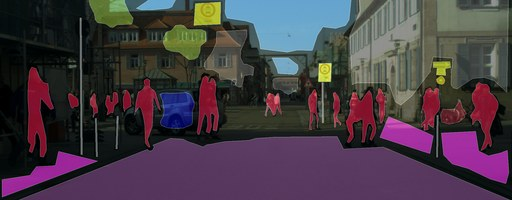
\includegraphics[width=\textwidth]{coarse_example.jpg}
		\caption{Coarse mask}
	\end{subfigure}
	\begin{subfigure}{.5\textwidth}
		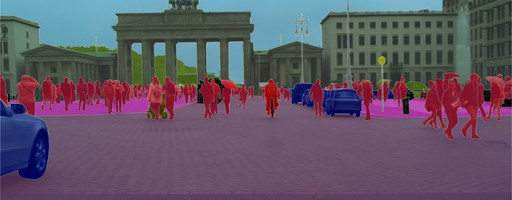
\includegraphics[width=\textwidth]{fine_example.jpg}
		\caption{Fine mask}
	\end{subfigure}
	\caption{Examples of coarse (a) and fine (b) mask annotations superimposed on the corresponding original images.}
	\label{fig:cityscapes}
\end{figure}

The cityscapes dataset offers tools that allow for the benchmarking of different models. One of the main metrics that is used in the evaluation of per-pixel semantic labelling of images is the Intersection over Union (IoU). This measures the overlap between the predicted segmentation and the ground truth and is expressed as the ratio: $\text{IoU} = \frac{TP}{TP + FP + FN}$ where TP, FP and FN are the numbers of true positive, false positive, and false negative pixels respectively. This formula gives a measure of how well the predicted labels agree with the true labels, across the entire testing set. Due to the fact that cityscapes offers two distinct granularities for semantic labelling (classes and categories), they report two separate IoU scores as IoU$_\text{category}$ and IoU$_\text{class}$. Pixels that are labelled as ``void" are excluded from these calculations. In our study, IoU scores refer exclusively to IoU$_\text{class}$, as we have only worked with that level of granularity.

Traditional IoU can be biased towards larger objects (which can dominate the score due to their size), hence another metric called iIoU is designed to provide a more balanced comparison, especially in street scenes where object size variability can be substantial. iIoU is defined as $\text{iIoU} = \frac{iTP}{iTP + FP + iFN}$. Here iTP are true positives that are weighted by the ratio of the class's average instance size to the size of the respective ground truth instance. False negatives are similarly adjusted based on the relative size of the object they belong to. The count of false positives remains unweighted, since these do not correspond to a specific instance size (they are areas that are incorrectly labelled as an object). Similarly to IoU, iIoU is reported in the Cityscapes website both for categories and classes to provide insight into the model's performance across different levels of semantic detail. We have deployed IoU and iIoU scores as a good performance metric for the evaluation of our models. 